\section{Результаты}
\subsection{Зависимость расстояния между экстремумами от времени, оставшегося до срыва разряда}

\begin{figure}[H]
	\begin{minipage}[H]{0.49\linewidth}
		\begin{center}
			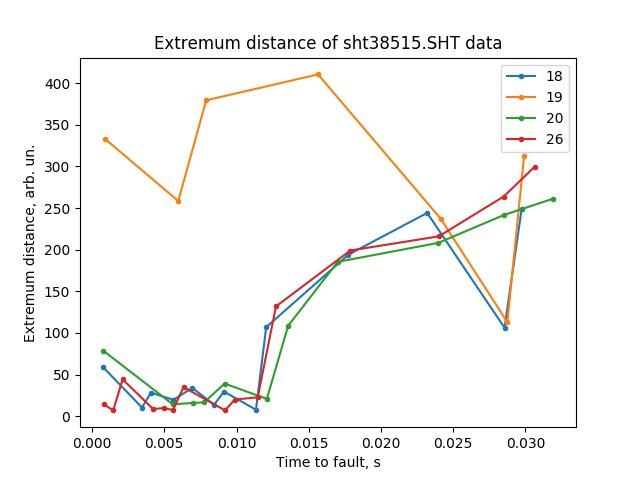
\includegraphics[width=\linewidth]{period_sht38515}
			\caption{sht38515}
		\end{center}
	\end{minipage}
	\hfill
	\begin{minipage}[H]{0.49\linewidth}
		\begin{center}
			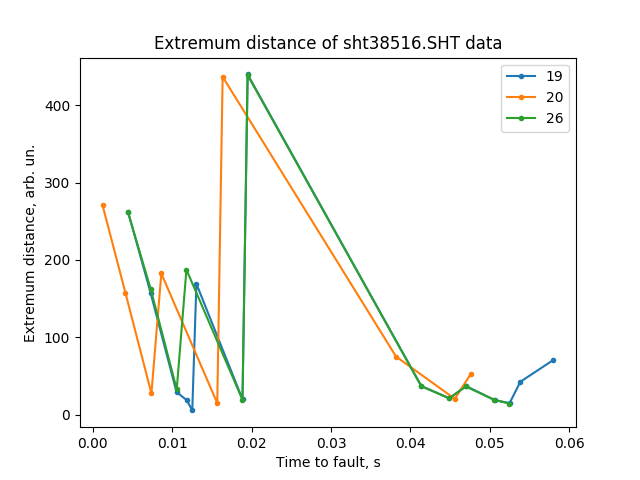
\includegraphics[width=\linewidth]{period_sht38516}
			\caption{sht38516}
		\end{center}
	\end{minipage}	
\end{figure}

\begin{figure}[H]
	\begin{minipage}[H]{0.49\linewidth}
		\begin{center}
			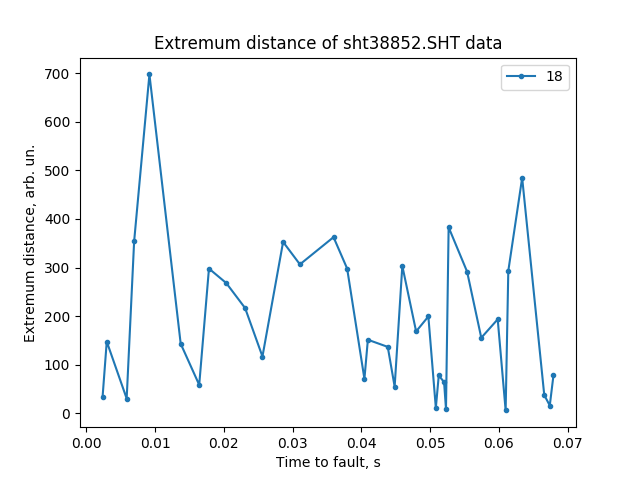
\includegraphics[width=\linewidth]{period_sht38852}
			\caption{sht38852}
		\end{center}
	\end{minipage}
	\hfill
	\begin{minipage}[H]{0.49\linewidth}
		\begin{center}
			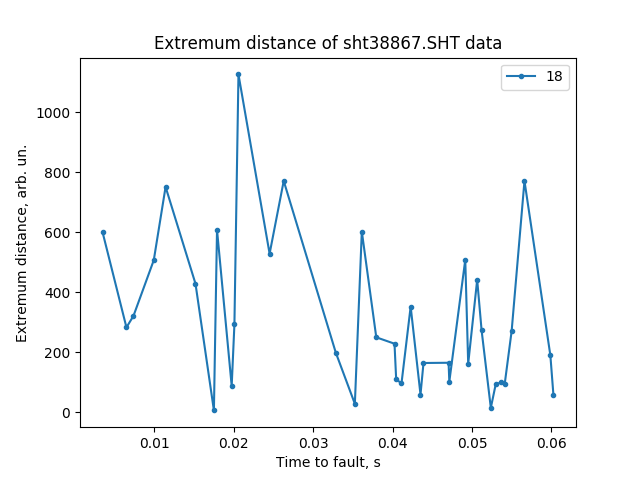
\includegraphics[width=\linewidth]{period_sht38867}
			\caption{sht38867}
		\end{center}
	\end{minipage}	
\end{figure}

\begin{figure}[H]
	\begin{minipage}[H]{0.49\linewidth}
		\begin{center}
			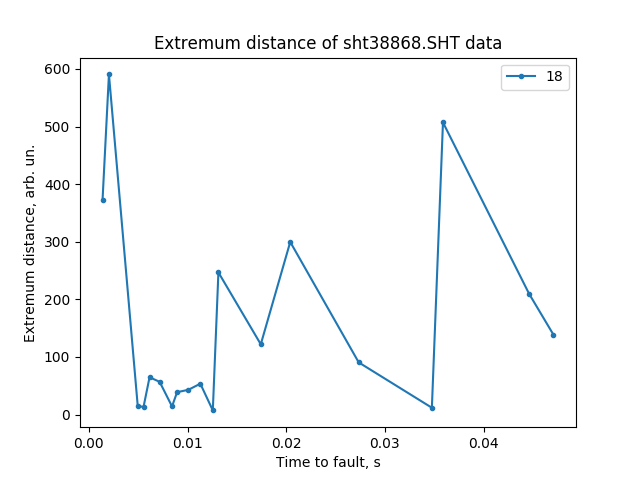
\includegraphics[width=\linewidth]{period_sht38868}
			\caption{sht38868}
		\end{center}
	\end{minipage}
	\hfill
	\begin{minipage}[H]{0.49\linewidth}
		\begin{center}
			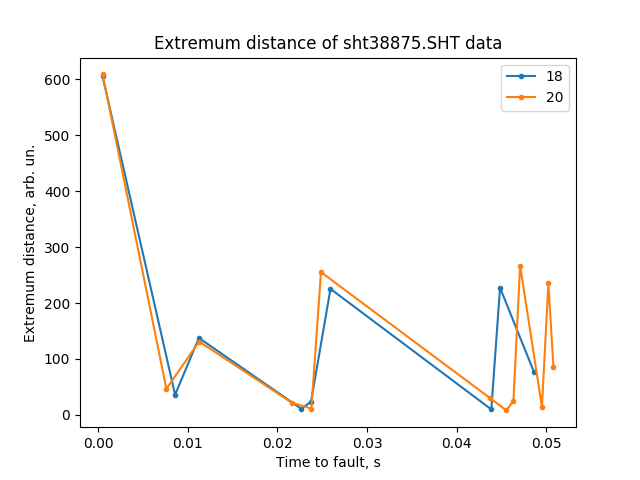
\includegraphics[width=\linewidth]{period_sht38875}
			\caption{sht38875}
		\end{center}
	\end{minipage}	
\end{figure}

\begin{figure}[H]
	\begin{minipage}[H]{0.49\linewidth}
		\begin{center}
			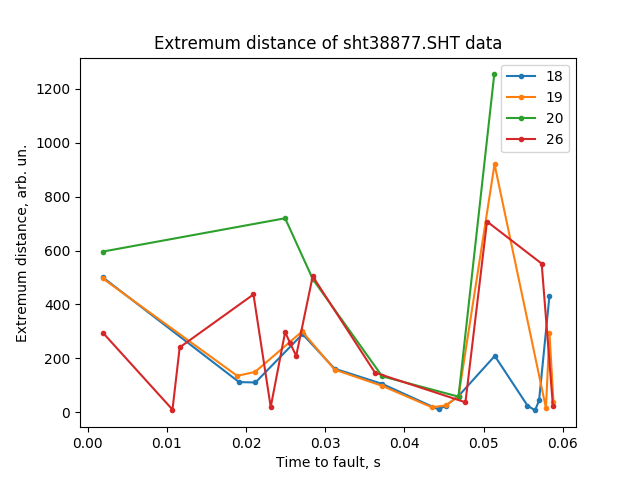
\includegraphics[width=\linewidth]{period_sht38877}
			\caption{sht38877}
		\end{center}
	\end{minipage}
	\hfill
	\begin{minipage}[H]{0.49\linewidth}
		\begin{center}
			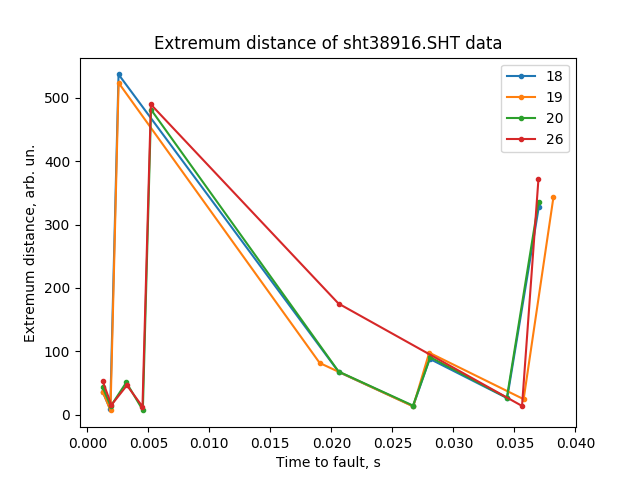
\includegraphics[width=\linewidth]{period_sht38916}
			\caption{sht38916}
		\end{center}
	\end{minipage}	
\end{figure}

\begin{figure}[H]
	\begin{center}
		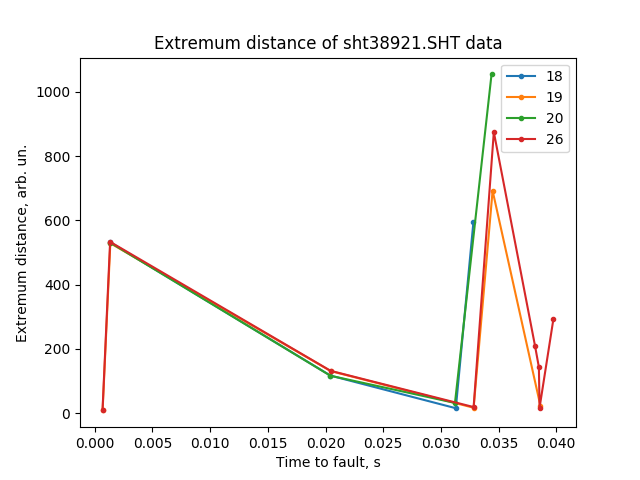
\includegraphics[width=0.5\linewidth]{period_sht38921}
		\caption{sht38921}
	\end{center}
\end{figure}

\subsection{Графики локальных минимумов частотных портретов}

\begin{figure}[H]
	\begin{minipage}[H]{0.49\linewidth}
		\begin{center}
			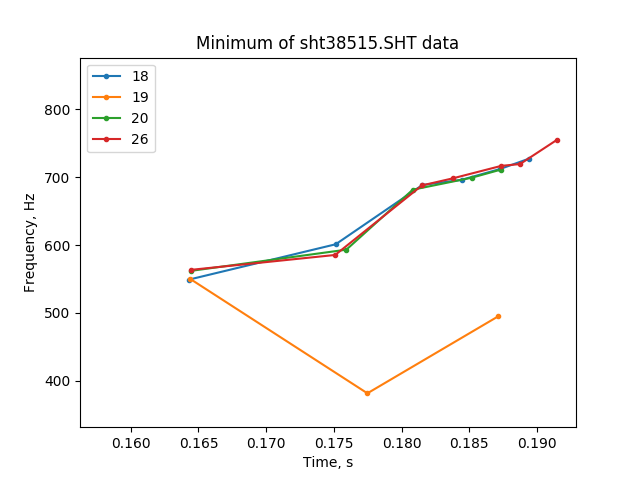
\includegraphics[width=\linewidth]{min_sht38515}
			\caption{sht38515}
		\end{center}
	\end{minipage}
	\hfill
	\begin{minipage}[H]{0.49\linewidth}
		\begin{center}
			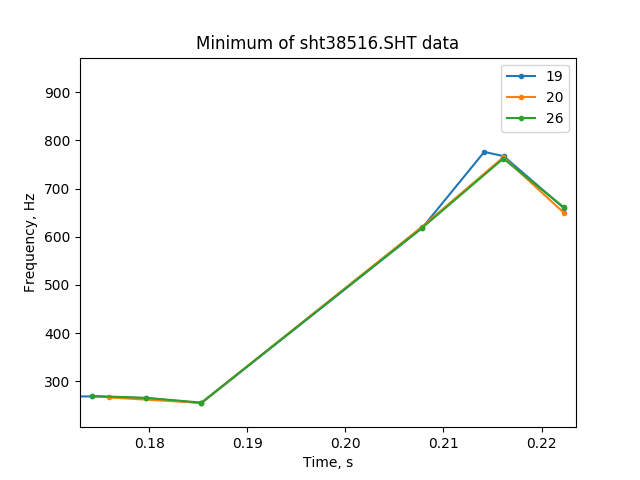
\includegraphics[width=\linewidth]{min_sht38516}
			\caption{sht38516}
		\end{center}
	\end{minipage}	
\end{figure}

\begin{figure}[H]
	\begin{minipage}[H]{0.49\linewidth}
		\begin{center}
			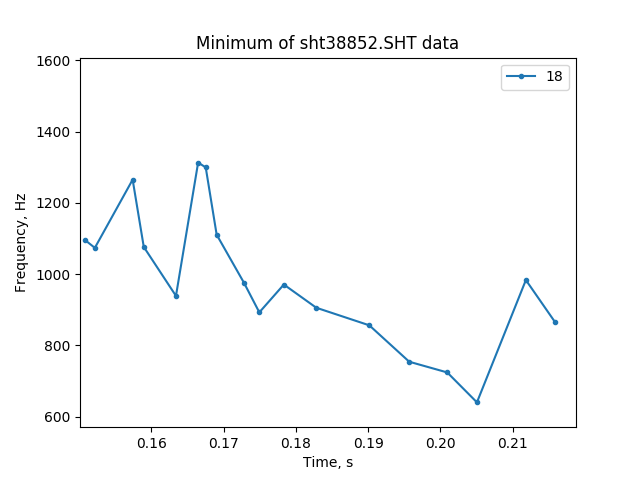
\includegraphics[width=\linewidth]{min_sht38852}
			\caption{sht38852}
		\end{center}
	\end{minipage}
	\hfill
	\begin{minipage}[H]{0.49\linewidth}
		\begin{center}
			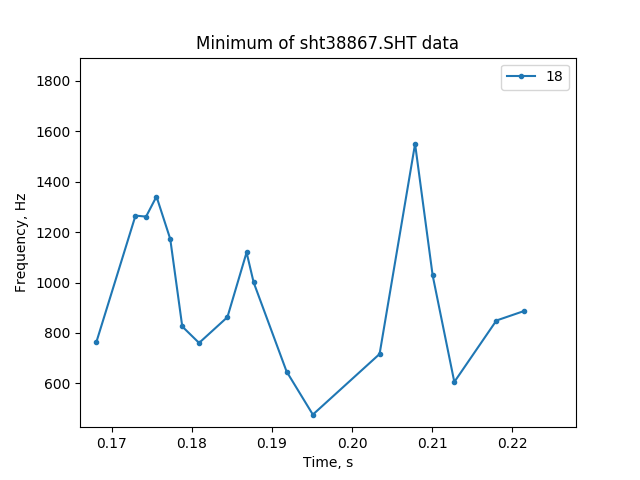
\includegraphics[width=\linewidth]{min_sht38867}
			\caption{sht38867}
		\end{center}
	\end{minipage}	
\end{figure}

\begin{figure}[H]
	\begin{minipage}[H]{0.49\linewidth}
		\begin{center}
			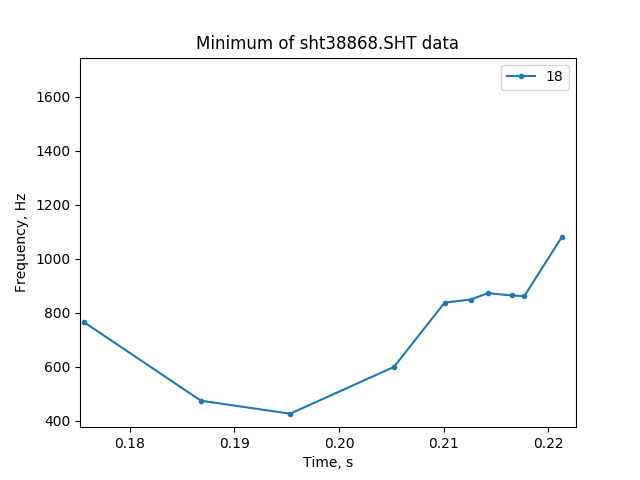
\includegraphics[width=\linewidth]{min_sht38868}
			\caption{sht38868}
		\end{center}
	\end{minipage}
	\hfill
	\begin{minipage}[H]{0.49\linewidth}
		\begin{center}
			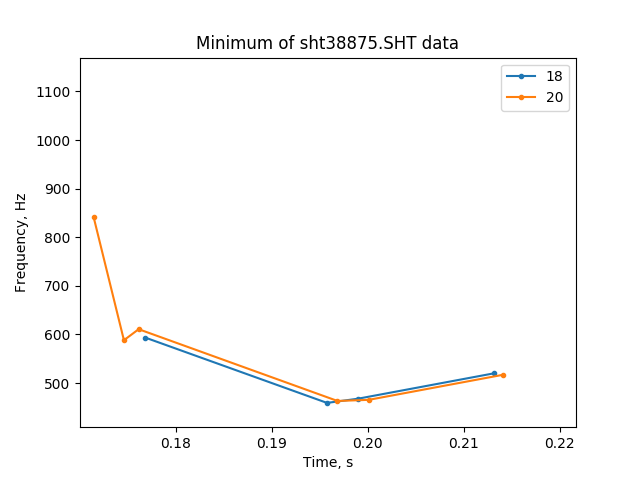
\includegraphics[width=\linewidth]{min_sht38875}
			\caption{sht38875}
		\end{center}
	\end{minipage}	
\end{figure}

\begin{figure}[H]
	\begin{minipage}[H]{0.49\linewidth}
		\begin{center}
			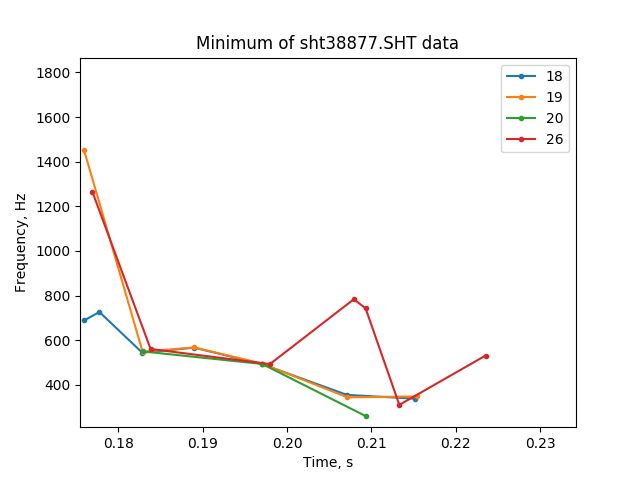
\includegraphics[width=\linewidth]{min_sht38877}
			\caption{sht38877}
		\end{center}
	\end{minipage}
	\hfill
	\begin{minipage}[H]{0.49\linewidth}
		\begin{center}
			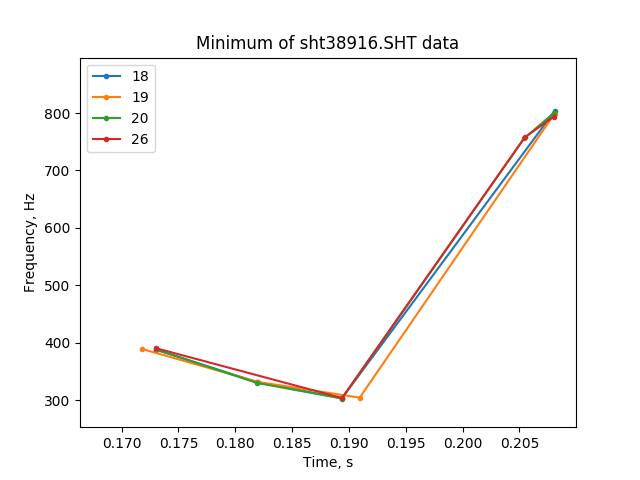
\includegraphics[width=\linewidth]{min_sht38916}
			\caption{sht38916}
		\end{center}
	\end{minipage}	
\end{figure}

\begin{figure}[H]
	\begin{center}
		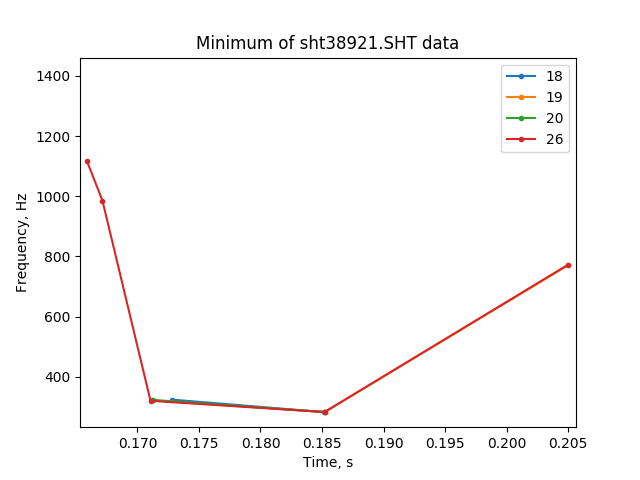
\includegraphics[width=0.5\linewidth]{min_sht38921}
		\caption{sht38921}
	\end{center}
\end{figure}

\subsection{Время от момента достижения <<дна>> частотной истории до срыва}

\begin{figure}[H]
	\begin{center}
		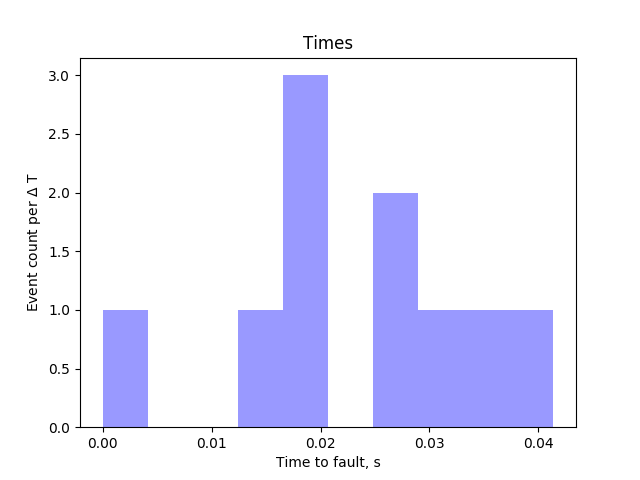
\includegraphics[width=0.5\linewidth]{times_sht}
		\caption{Время до срыва. Выборка для всех рассмотренных экспериментов. 18 датчик}
	\end{center}
\end{figure}

\begin{table}[H]
\begin{center}
	\begin{tabular}{|c|c|}
		\hline
		$E(T)$ & $D(T)$ \\
		\hline
		0.02 & 0.01 \\
		\hline
	\end{tabular}
	\caption{Среднее время до срыва и дисперсия по всем экспериментам для 18 датчика}
	\label{table:dt}
\end{center}
\end{table}

Нижележащие графики и таблицы не были заявлены в разделе ~\hyperref[analysis]{<<анализ данных>>}, однако интерес к и построению возник во время анализа полученных выше графиков. Описание смотрите в разделе ~\hyperref[discuss]{<<Обсуждение>>}.

\begin{figure}[H]
	\begin{center}
		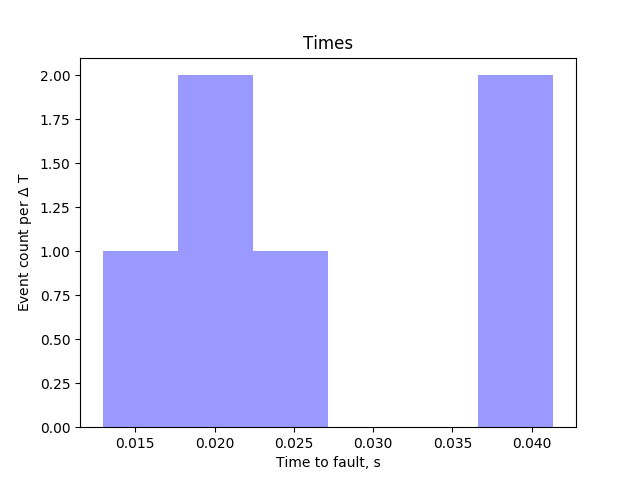
\includegraphics[width=0.5\linewidth]{times_sht2}\label{pic:min2}
		\caption{Время до срыва. Выборка для экспериментов 38815, 38516, 38868, 38875, 38916, 38921}
	\end{center}
\end{figure}

\begin{table}[H]
	\begin{center}
		\begin{tabular}{|c|c|}
			\hline
			$E(T)$ & $D(T)$ \\
			\hline
			0.026 & 0.009 \\
			\hline
		\end{tabular}
		\caption{Среднее время до срыва и дисперсия по экспериментам 38815, 38516, 38868, 38875, 38916, 38921 для 18 датчика}
		\label{table:dt1}
	\end{center}
\end{table}

\begin{figure}[H]
	\begin{center}
		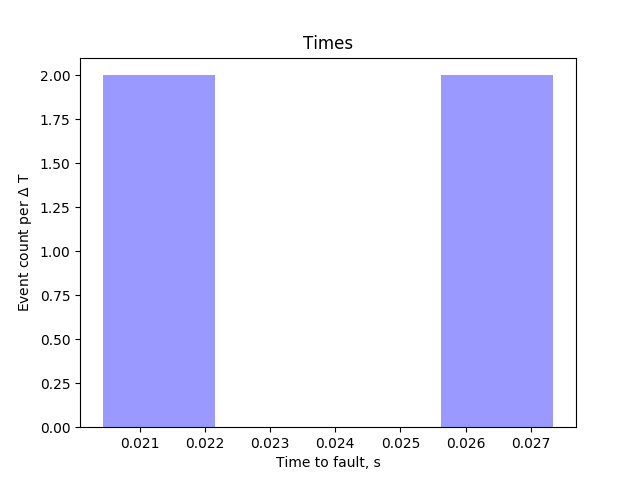
\includegraphics[width=0.5\linewidth]{times_sht3}\label{pic:min3}
		\caption{Время до срыва. Выборка для экспериментов 38815, 38516, 38868, 38875, 38916, 38921}
	\end{center}
\end{figure}

\begin{table}[H]
	\begin{center}
		\begin{tabular}{|c|c|}
			\hline
			$E(T)$ & $D(T)$ \\
			\hline
			0.023 & 0.003 \\
			\hline
		\end{tabular}
		\caption{Среднее время до срыва и дисперсия по экспериментам 38868, 38875, 38916, 38921 для 18 датчика}
		\label{table:dt3}
	\end{center}
\end{table}